\documentclass[UTF8,aspectratio=169,11pt]{ctexbeamer}

\usetheme{default}
\usefonttheme{professionalfonts}
\usepackage{amsmath,amssymb}
\usepackage{booktabs}
\usepackage{array}
\usepackage{graphicx}
\usepackage{xcolor}
\usepackage{tikz}
\usepackage{fontspec}
\usetikzlibrary{positioning}

\definecolor{paperblue}{HTML}{1F4E79}
\definecolor{papergray}{HTML}{4B5563}
\definecolor{lightgray}{HTML}{E5E7EB}
\definecolor{softblue}{HTML}{EAF2F8}

\setbeamercolor{background canvas}{bg=white}
\setbeamercolor{normal text}{fg=black,bg=white}
\setbeamercolor{frametitle}{fg=paperblue,bg=white}
\setbeamercolor{title}{fg=paperblue,bg=white}
\setbeamercolor{structure}{fg=paperblue}
\setbeamercolor{itemize item}{fg=paperblue}
\setbeamercolor{itemize subitem}{fg=papergray}
\setbeamertemplate{navigation symbols}{}
\setbeamertemplate{headline}{}
\setbeamertemplate{footline}{%
  \leavevmode%
  \hbox{%
    \begin{beamercolorbox}[wd=.78\paperwidth,ht=2.5ex,dp=1ex,leftskip=0.6cm]{author in head/foot}
      \scriptsize\color{papergray} Map Coloring Lab 3
    \end{beamercolorbox}%
    \begin{beamercolorbox}[wd=.22\paperwidth,ht=2.5ex,dp=1ex,rightskip=0.6cm plus1fil]{date in head/foot}
      \scriptsize\color{papergray}\hfill \insertframenumber/\inserttotalframenumber
    \end{beamercolorbox}}%
}

\setbeamertemplate{itemize item}{\raise0.15ex\hbox{\scriptsize$\blacktriangleright$}}
\setlength{\parskip}{0.2em}

\newcommand{\slidekicker}[1]{\vspace{-0.2em}{\small\color{papergray}#1}\vspace{0.35em}}
\newcommand{\claim}[1]{{\Large\bfseries\color{paperblue}#1}}
\newcommand{\metric}[2]{%
  \begin{minipage}[t]{0.28\linewidth}
    {\huge\bfseries\color{paperblue}#1}\\[-0.1em]
    {\small\color{papergray}#2}
  \end{minipage}
}
\newcommand{\algo}[1]{\textsc{#1}}

\title{地图填色：从暴力回溯到 DSATUR 与 TabuCol}
\subtitle{5 分钟 oral：只讲模型、优化与复现实验结果}
\author{实验3：回溯法（地图填色问题）}
\date{}

\begin{document}

\begin{frame}[plain]
  \vspace{1.0cm}
  {\Huge\bfseries\color{paperblue}地图填色}\\[0.25cm]
  {\LARGE\bfseries 从暴力回溯到 DSATUR 与 TabuCol}\\[0.55cm]
  {\large\color{papergray}一个可复现的图着色实验流水线：建模、剪枝优化、局部搜索、结果验证}\\[1.0cm]
  \begin{center}
    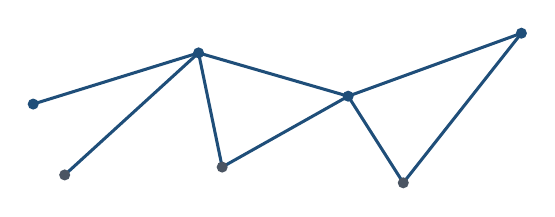
\begin{tikzpicture}[x=1cm,y=1cm]
      \draw[paperblue, line width=1.1pt] (0,0) -- (2.1,0.65) -- (4.0,0.1) -- (6.2,0.9);
      \draw[paperblue, line width=1.1pt] (0.4,-0.9) -- (2.1,0.65) -- (2.4,-0.8) -- (4.0,0.1);
      \draw[paperblue, line width=1.1pt] (4.0,0.1) -- (4.7,-1.0) -- (6.2,0.9);
      \foreach \x/\y/\c in {0/0/paperblue,2.1/0.65/paperblue,4.0/0.1/paperblue,6.2/0.9/paperblue,0.4/-0.9/papergray,2.4/-0.8/papergray,4.7/-1.0/papergray}
        \fill[\c] (\x,\y) circle (2.0pt);
    \end{tikzpicture}
  \end{center}
  \vfill
  {\small\color{papergray}白底极简版式；所有结果以冲突边数为合法性判据}
\end{frame}

\begin{frame}{核心问题：把“地图”压缩成一个可验证模型}
  \slidekicker{不讲四色定理常识；直接讲我设计的实验对象与评价指标}
  \claim{区域邻接关系 $\Rightarrow$ 图的 $k$-着色约束满足问题}

  \vspace{0.4cm}
  \begin{columns}[T,onlytextwidth]
    \begin{column}{0.49\textwidth}
      \begin{align*}
        G&=(V,E),\quad C=\{1,\ldots,k\}\\
        f&:V\rightarrow C\\
        (u,v)\in E&\Rightarrow f(u)\ne f(v)
      \end{align*}
    \end{column}
    \begin{column}{0.48\textwidth}
      \small
        \begin{tabular}{@{}p{0.22\linewidth}p{0.70\linewidth}@{}}
        \toprule
        设计项 & 本实验实现 \\
        \midrule
        输入 & 小图邻接、DIMACS .col、随机平面图 \\
        目标 & 给定颜色数下构造合法染色 \\
        判据 & 冲突边数 $=0$ \\
        输出 & 每个顶点的颜色编号 CSV \\
        \bottomrule
      \end{tabular}
    \end{column}
  \end{columns}

  \vspace{0.45cm}
  \begin{center}
    \metric{$0$}{合法解冲突边数}\hfill
    \metric{$450$}{基准图顶点数}\hfill
    \metric{$20\sim300$}{平面图规模}
  \end{center}
\end{frame}

\begin{frame}{优化一：从固定顺序暴力回溯到 DSATUR}
  \slidekicker{复现 Brélaz 的 DSATUR 思想，并把它接入回溯与前向检查}
  \begin{columns}[T,onlytextwidth]
    \begin{column}{0.45\textwidth}
      \small
      \begin{tabular}{@{}p{0.32\linewidth}p{0.58\linewidth}@{}}
        \toprule
        方法 & 关键问题 \\
        \midrule
        暴力回溯 & 固定顶点顺序，最坏枚举 $k^n$ \\
        DSATUR & 先处理约束最紧顶点 \\
        前向检查 & 某邻居无可用色时立即剪枝 \\
        \bottomrule
      \end{tabular}

      \vspace{0.55cm}
      \small
      \textbf{饱和度定义}
      \[
        sat(v)=|\{f(u)\mid u\in N(v), f(u)\ne \varnothing\}|
      \]
    \end{column}
    \begin{column}{0.52\textwidth}
      \small
      \begin{tabular}{@{}r p{0.75\linewidth}@{}}
        \toprule
        行 & DSATUR-Backtracking 核心流程 \\
        \midrule
        1 & 维护每个未着色顶点的可用颜色集合 \\
        2 & 选择 $sat(v)$ 最大的未着色顶点 \\
        3 & 并列时选择度数 $\deg(v)$ 最大者 \\
        4 & 尝试颜色 $c$，并临时删除邻居域中的 $c$ \\
        5 & 若产生空颜色域，则立即回溯 \\
        6 & 若全部顶点着色完成，返回合法解 \\
        \bottomrule
      \end{tabular}
    \end{column}
  \end{columns}

  \vspace{0.35cm}
  \claim{优化点不是改变问题，而是改变搜索顺序：更早遇到矛盾，更少进入无效分支。}
\end{frame}

\begin{frame}{优化二：450 顶点实例用 TabuCol 求可行解}
  \slidekicker{精确回溯不适合直接处理 le450；改用局部搜索快速构造 0 冲突解}
  \begin{columns}[T,onlytextwidth]
    \begin{column}{0.50\textwidth}
      \small
      \begin{tabular}{@{}r p{0.72\linewidth}@{}}
        \toprule
        行 & TabuCol 局部搜索核心流程 \\
        \midrule
        1 & 贪心生成初始 $k$-着色，允许冲突 \\
        2 & 只在冲突顶点集合中选择移动 \\
        3 & 评价移动 $\Delta =$ 新冲突数 $-$ 旧冲突数 \\
        4 & 最优移动若被禁忌，只有优于历史最优时允许 \\
        5 & 更新颜色与禁忌表，直到冲突边数为 0 \\
        \bottomrule
      \end{tabular}
    \end{column}
    \begin{column}{0.47\textwidth}
      \begin{center}
        \begin{tikzpicture}[node distance=0.34cm, every node/.style={font=\scriptsize}]
          \node[draw=paperblue, rounded corners=1pt, line width=0.8pt, minimum width=4.0cm, minimum height=0.48cm] (a) {贪心初始解};
          \node[draw=paperblue, rounded corners=1pt, line width=0.8pt, minimum width=4.0cm, minimum height=0.48cm, below=of a] (b) {定位冲突顶点};
          \node[draw=paperblue, rounded corners=1pt, line width=0.8pt, minimum width=4.0cm, minimum height=0.48cm, below=of b] (c) {选择最优非禁忌移动};
          \node[draw=paperblue, rounded corners=1pt, line width=0.8pt, minimum width=4.0cm, minimum height=0.48cm, below=of c] (d) {更新禁忌表};
          \node[draw=paperblue, rounded corners=1pt, line width=0.8pt, minimum width=4.0cm, minimum height=0.48cm, below=of d] (e) {冲突边数 $=0$};
          \draw[->, paperblue, line width=0.8pt] (a) -- (b);
          \draw[->, paperblue, line width=0.8pt] (b) -- (c);
          \draw[->, paperblue, line width=0.8pt] (c) -- (d);
          \draw[->, paperblue, line width=0.8pt] (d) -- (e);
        \end{tikzpicture}
      \end{center}
    \end{column}
  \end{columns}
  \vspace{0.15cm}
  {\scriptsize\color{papergray}定位：DSATUR 做确定性验证；TabuCol 做大规模给定颜色数下的快速可行染色。}
\end{frame}

\begin{frame}{复现实验：暴力回溯 vs DSATUR}
  \slidekicker{首解可能很快，但完整搜索空间暴露了暴力法的指数风险}
  \small
  \begin{tabular}{@{}lrrrrr@{}}
    \toprule
    数据 & 顶点 & 暴力赋值 & DSATUR赋值 & 暴力完整空间 & 外推/s \\
    \midrule
    小规模地图 & 9 & 19 & 9 & $2.621\times10^5$ & $2.580\times10^{-1}$ \\
    平面图 $n=20$ & 20 & 51 & 20 & $1.100\times10^{12}$ & $6.985\times10^5$ \\
    平面图 $n=32$ & 32 & 78 & 32 & $1.845\times10^{19}$ & $1.102\times10^{13}$ \\
    \bottomrule
  \end{tabular}

  \vspace{0.55cm}
  \begin{columns}[T,onlytextwidth]
    \begin{column}{0.49\textwidth}
      \claim{DSATUR 的优势体现在搜索节点数，而不只是一两个样例的运行时间。}
    \end{column}
    \begin{column}{0.48\textwidth}
      \small
      \begin{itemize}
        \item 暴力法：固定顺序，完整空间为 $4^n$
        \item DSATUR：动态选点，实验中赋值次数约等于 $n$
        \item 外推只用于说明指数增长趋势，不当作实际运行时间
      \end{itemize}
    \end{column}
  \end{columns}
\end{frame}

\begin{frame}{复现实验：le450 基准与随机平面图}
  \slidekicker{所有最终结果都用冲突边数校验；合法标准统一为 conflict = 0}
  \begin{columns}[T,onlytextwidth]
    \begin{column}{0.52\textwidth}
      \small
      \begin{tabular}{@{}lrrrr@{}}
        \toprule
        数据 & 顶点 & 边 & 颜色 & 耗时/s \\
        \midrule
        le450\_5a & 450 & 5714 & 5 & 1.104681 \\
        le450\_15b & 450 & 8169 & 15 & 2.501488 \\
        le450\_25a & 450 & 8260 & 25 & 0.007555 \\
        \bottomrule
      \end{tabular}
      \vspace{0.25cm}

      {\small\color{papergray}三组均成功，冲突边数均为 0。}
    \end{column}
    \begin{column}{0.45\textwidth}
      \small
      \begin{tabular}{@{}rrrr@{}}
        \toprule
        $n$ & 边数 & 耗时/s & 冲突 \\
        \midrule
        20 & 54 & 0.000280 & 0 \\
        80 & 234 & 0.001980 & 0 \\
        160 & 474 & 0.005360 & 0 \\
        300 & 894 & 0.020500 & 0 \\
        \bottomrule
      \end{tabular}
      \vspace{0.25cm}

      {\small\color{papergray}随机平面图全部 4 色成功。}
    \end{column}
  \end{columns}

  \vspace{0.55cm}
  \claim{颜色数越宽松，局部搜索越容易收敛；边数更多、颜色更少时约束更强。}
\end{frame}

\begin{frame}{5 分钟汇报结论：我做了什么，优化在哪里}
  \slidekicker{结束页只保留可答辩的三点}
  \begin{enumerate}
    \item \textbf{模型设计}：统一把手工地图、DIMACS .col 和随机平面图表示为无向图；用冲突边数 $=0$ 作为唯一合法性判据。
    \item \textbf{算法优化}：从暴力回溯的固定顺序，改为 DSATUR 的饱和度优先和前向检查；大图使用 TabuCol 避免精确搜索爆炸。
    \item \textbf{复现结果}：小图、随机平面图、三个 le450 数据全部得到 0 冲突解；DSATUR 降低搜索赋值次数，TabuCol 在 450 点图上快速收敛。
  \end{enumerate}

  \vspace{0.55cm}
  \small\color{papergray}
  参考：Brélaz, CACM 1979；Robertson--Sanders--Seymour--Thomas, JCTB 1997；Leighton, J. Res. NBS 1979。
\end{frame}

\end{document}
